\documentclass[sigconf,nonacm]{acmart}
\settopmatter{printacmref=false,printfolios=true}
\setcopyright{none}
\usepackage{booktabs}
\usepackage{graphicx}
\usepackage{amsmath}
\usepackage{siunitx}
\title{Making Data Movement Visible: An Illustrative Study of IO-Aware Attention}
\subtitle{An English Envoi Demonstration with Synthetic Data}
\author{Envoi Demonstration}
\affiliation{\institution{Illustrative manuscript, not a research affiliation}\city{}\country{}}
\renewcommand{\shortauthors}{Envoi Demonstration}
\begin{document}
\begin{abstract}
Attention performance depends on both arithmetic and the movement of intermediate data. A useful systems discussion must separate algorithmic structure, an explicit performance model, and measurements on an actual implementation. This demonstration develops a transparent, reproducible numerical model for comparing a materialized attention schedule with a tiled schedule. It examines sequence length, head dimension, bandwidth, compute efficiency, and temporary workspace, and connects the resulting plots to practical experimental design. Every numerical result in this manuscript is synthetic: no GPU kernel was implemented, no device was benchmarked, and no speedup is presented as a measured result. The contribution is an auditable example of systems reasoning and a complete authoring artifact, including source files, figures, tables, cross-references, and a real BibTeX bibliography. The model illustrates how apparently strong local improvements can be limited by launch overhead, arithmetic throughput, or the fraction of execution spent outside attention. It also identifies the measurements that would be required before making a hardware-performance claim.
\end{abstract}
\keywords{attention, data movement, performance modeling, synthetic data, reproducibility}
\maketitle
\section{Introduction}
\label{sec:intro}
Long-context model execution makes the memory hierarchy difficult to ignore. An implementation can perform mathematically familiar operations yet exhibit very different runtime behavior depending on which tensors are stored, when they are reused, and how much work is exposed to the device. Describing a workload only by its floating-point operation count therefore leaves an important part of the systems problem unspecified. The missing description is a schedule: which intermediate values are produced together, which remain nearby, and which travel through a more expensive level of memory.

The Transformer architecture established attention as a central sequence-modeling operation~\cite{vaswani2017attention}. Subsequent IO-aware work reorganized attention computation around tiling and reuse, rather than treating the memory traffic of a straightforward schedule as unavoidable~\cite{dao2022flashattention}. These developments motivate a practical question for readers of performance papers: what evidence distinguishes a reduction in traffic, a reduction in peak allocation, and an improvement in end-to-end time? The three quantities are related but cannot be substituted for one another.

This manuscript addresses that question through an explicitly synthetic study. Its purpose is not to introduce a new attention kernel. It provides a small model whose assumptions can be inspected, whose figures can be regenerated, and whose limitations are visible next to its conclusions. The model assigns arithmetic and byte counts to two abstract schedules and combines them with hypothetical device parameters. The resulting curves are numerical consequences of those assignments. They are not estimates calibrated to a particular accelerator, and they are not reproductions of published benchmark results.

The distinction matters because a convincing-looking graph can conceal several different claims. A smooth increase in speedup might result from improved reuse, but it might also follow automatically from a chosen denominator. A low workspace curve might exclude an allocation that a real runtime cannot avoid. A threshold at which one schedule becomes faster might move when launch latency, batching, or synchronization is included. Keeping the equations and the plotting data in the same project makes these possibilities easier to examine.

\subsection{Questions and intended use}
We organize the study around four questions. First, how does an explicit quadratic intermediate affect modeled memory traffic and workspace as sequence length grows? Second, when does reducing that traffic stop helping because arithmetic becomes the active constraint? Third, which assumptions move the crossover between the two abstract schedules? Fourth, what experimental protocol would be necessary to turn the illustration into a defensible implementation study?

A reader can use the artifact at three levels. At the first level, the figures offer a visual explanation of data movement. At the second, the equations expose a compact performance model that can be challenged or replaced. At the third, the project is a working authoring example: citations are resolved by BibTeX, figures are genuine vector graphics, and the preview is generated by a real LaTeX engine. None of these software properties establishes the truth of a hardware claim; they make the artifact easier to audit.

The remainder of the paper separates these levels deliberately. Section~\ref{sec:background} introduces the computational context. Sections~\ref{sec:model} and~\ref{sec:design} specify the model and its artifact organization. Sections~\ref{sec:evaluation} and~\ref{sec:sensitivity} interpret the synthetic results. Section~\ref{sec:discussion} explains how a future measured study would need to differ. The appendix records additional checks and reporting decisions so that the example can be extended without losing the distinction between evidence and illustration.

\section{Background and Related Work}
\label{sec:background}
For a single attention head, let $Q$, $K$, and $V$ contain $N$ token vectors of dimension $d$. Ignoring masking for the moment, scaled dot-product attention is
\begin{equation}
 O=\operatorname{softmax}(QK^{\mathsf T}/\sqrt{d})V.
 \label{eq:attention}
\end{equation}
The expression specifies the desired result, not the storage policy. A materialized schedule can form a score matrix, normalize it, and then multiply by the values. A tiled schedule can process smaller regions while maintaining the information needed to combine their contributions. The conceptual difference is the lifetime of intermediate data, not a change to the definition in Equation~\ref{eq:attention}.

\subsection{Exactness, scheduling, and numerical behavior}
FlashAttention studies exact attention through an IO-aware tiled algorithm that reduces transfers between GPU memory levels~\cite{dao2022flashattention}. FlashAttention-2 further examines work partitioning and parallelism~\cite{dao2023flashattention2}. We use these works to motivate two distinct concerns: reducing bytes moved and using the available arithmetic resources effectively. We do not copy their performance numbers into the synthetic dataset, and our two abstract schedules are not faithful simulators of either implementation.

Mathematical exactness also needs careful wording. Reordering finite-precision operations may change rounding even when an algorithm evaluates the same mathematical expression. A real correctness study should state the reference precision, tolerated error, and distributions of tested inputs. The absence of an approximation in the mathematical formulation does not remove the need for numerical validation. This paper models time and storage only; it makes no numerical-accuracy claim about executable attention code.

\subsection{Training, prefill, and decoding}
Attention appears in different execution regimes. A full sequence computation exposes a different shape from generating one token while reading a growing cache. Likewise, backward computation has different intermediate requirements from forward-only execution. Our main model describes a simplified forward full-sequence workload. It should not be read as a model of autoregressive decoding, complete training steps, or a production serving system.

PagedAttention addresses key--value cache management and sharing in language-model serving~\cite{kwon2023pagedattention}. Its context helps explain why an attention microbenchmark is not a serving benchmark. A service must also manage admission, batching, memory fragmentation, and request completion. A schedule that improves one dense attention operation can leave those system-level constraints unchanged. Conversely, better cache management can improve useful concurrency without changing the arithmetic expression for an individual head.

\subsection{Three quantities that should not be conflated}
Traffic is the amount of data transferred over a specified boundary during execution. Workspace is the maximum temporary storage simultaneously allocated under a stated lifetime model. Runtime is the duration of an operation under a measurement boundary. A tensor may be allocated once and read many times, so traffic can substantially exceed allocation size. A reduction in workspace may permit a larger batch, but the resulting throughput improvement depends on scheduling and the rest of the model.

We keep these quantities separate in both the notation and the artifact. Traffic expressions use bytes transferred; workspace curves use bytes resident; time curves use seconds. The units are converted only at plot boundaries, with binary units for workspace and decimal units for bandwidth. This bookkeeping is mundane but necessary: an unexplained factor of two can be a unit conversion, a second materialized tensor, or a genuinely different algorithm. Figure~\ref{fig:schedule} summarizes the abstraction used throughout the manuscript.

\begin{figure*}[t]
 \centering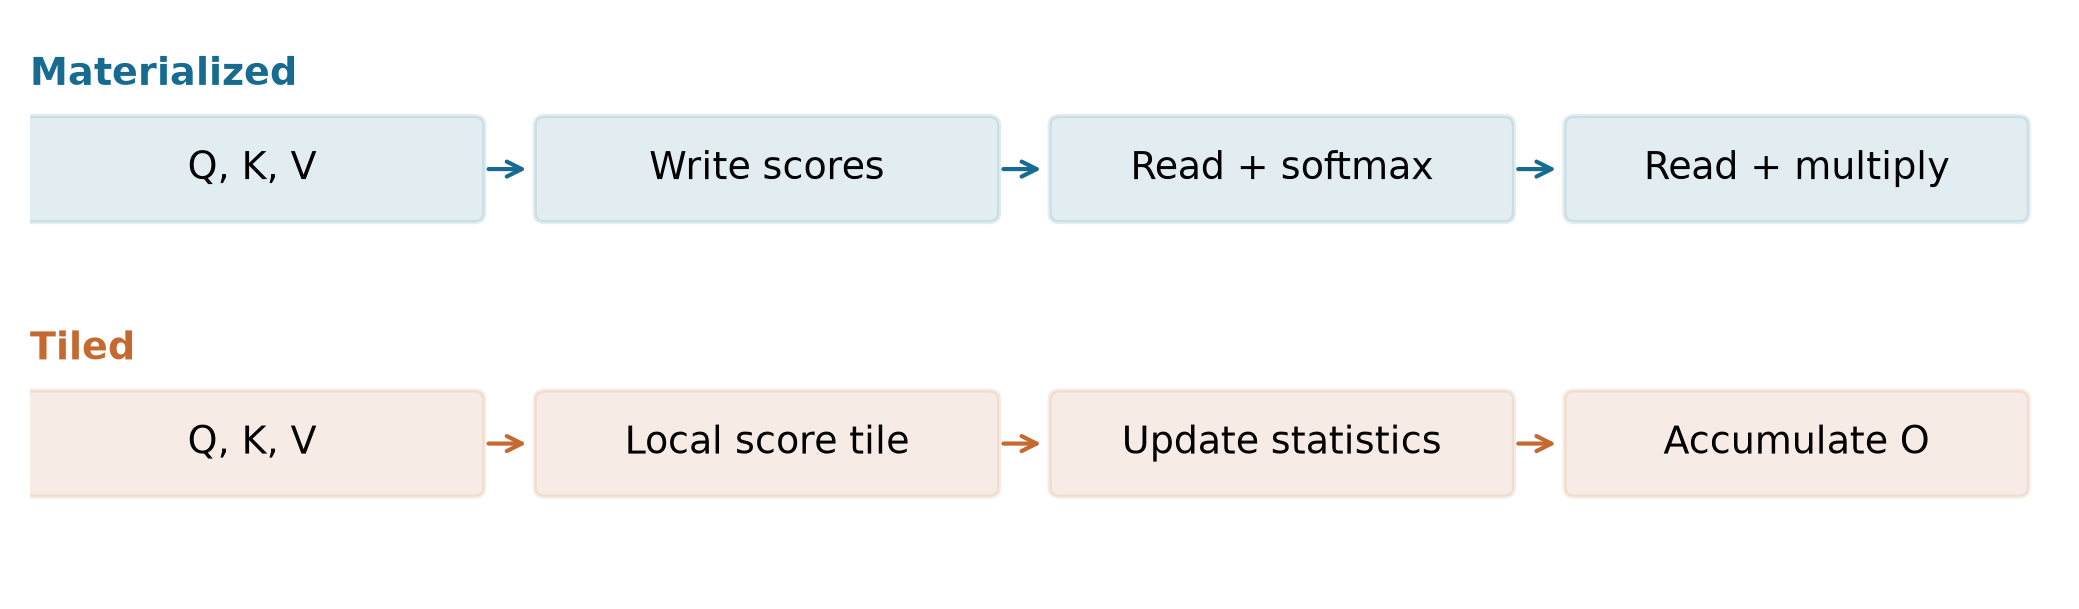
\includegraphics[width=.94\textwidth]{assets/schedule.png}
 \caption{Abstract schedules used in the demonstration. These diagrams explain intermediate lifetimes; they are not GPU implementation traces. Both schedules target the same mathematical attention expression.}
 \label{fig:schedule}
\end{figure*}

\section{A Transparent Synthetic Model}
\label{sec:model}
We consider one head and assign both schedules the same leading arithmetic count,
\begin{equation}
 F(N,d)=4N^2d.
 \label{eq:flops}
\end{equation}
The coefficient represents two matrix products in a deliberately compact convention. It excludes softmax arithmetic, address calculation, masking, and auxiliary instructions. Using the same count isolates the influence of the traffic assumptions, but it is not an assertion that real schedules perform identical instruction sequences.

The traffic surrogates are
\begin{align}
 B_{\mathrm{mat}}(N,d)&=8N^2+8Nd,\\
 B_{\mathrm{tile}}(N,d)&=0.5N^2+8Nd.
 \label{eq:bytes}
\end{align}
Both expressions are in bytes. The coefficients are selected for illustration, not derived from a particular published implementation. The quadratic term represents repeated handling of pairwise intermediates, while the shared linear term represents input and output movement. Retaining a smaller quadratic term for the tiled case avoids pretending that this simplified model captures every reuse opportunity or that data movement disappears completely.

\subsection{Runtime and resource parameters}
Let $P$ be a hypothetical peak arithmetic rate, $W$ a hypothetical peak bandwidth, and $\eta_c$ and $\eta_b$ their respective effective fractions. For schedule $s$, we define
\begin{equation}
 T_s=\tau+\max\left(\frac{F}{\eta_cP},\frac{B_s}{\eta_bW}\right).
 \label{eq:time}
\end{equation}
The maximum treats arithmetic and transfer as perfectly overlappable at the level of this model. This is an optimistic abstraction. A sum would be more conservative for serialized work, while a detailed simulator would need dependency and concurrency information. The launch term $\tau$ makes small-workload behavior explicit instead of forcing every curve through the origin.

The baseline parameters appear in Table~\ref{tab:parameters}. They describe a hypothetical device, not a named GPU. Their round values are intended to simplify inspection. Effective rates are separate from peak rates so that sensitivity experiments can vary efficiency without changing the nominal device. All later conclusions are conditional on these parameters and the byte-count surrogates.

\begin{table}[t]
 \caption{Baseline assumptions. Every value is synthetic and is not a device specification.}
 \label{tab:parameters}\centering
 \begin{tabular}{lr}\toprule
 Parameter & Illustrative value\\\midrule
 Peak arithmetic $P$ & $120\times10^{12}$ FLOP/s\\
 Peak bandwidth $W$ & $1.2\times10^{12}$ byte/s\\
 Arithmetic fraction $\eta_c$ & 0.60\\
 Bandwidth fraction $\eta_b$ & 0.65\\
 Launch term $\tau$ & $30\,\mu$s\\
 Baseline head dimension $d$ & 64\\
 Tile dimensions $(B_r,B_c)$ & $(128,128)$\\\bottomrule
 \end{tabular}
\end{table}

\subsection{Workspace is a separate model}
We assign the materialized schedule a temporary workspace of $4N^2$ bytes. The tiled surrogate receives $4Nd+8B_rB_c+16N$ bytes. The first tiled term represents an output-sized accumulator, the second a fixed tile allocation, and the last per-row statistics. These are explicit accounting choices. They exclude model parameters, permanent input tensors, allocator bookkeeping, and any backward-pass state.

This separation prevents a common interpretive shortcut. Equation~\ref{eq:bytes} may predict large traffic even when the workspace remains small, because a buffer can be reused repeatedly. Conversely, a persistent allocation might occupy considerable space while being accessed only a few times. The model therefore reports workspace and time in different plots rather than using one as a proxy for the other.

\subsection{Derived quantities and interpretive limits}
The synthetic speedup is $S=T_{\mathrm{mat}}/T_{\mathrm{tile}}$. It compares model outputs under the same parameter tuple. It is neither a confidence interval nor an estimate from repeated trials. Arithmetic intensity is $I_s=F/B_s$, with FLOP per byte as its unit. A crossover occurs when this intensity meets the ratio of effective arithmetic rate to effective bandwidth, but the launch term can still dominate total time on either side.

The formulas intentionally omit several important effects. Cache residency, register pressure, tile occupancy, instruction-level overhead, and device power behavior do not appear. A curve cannot reveal a phenomenon that the model has no variable for. Later sections use sensitivity analyses to show how some assumptions matter; they do not claim to repair every omission. The artifact is useful precisely because a reader can see where its reasoning ends.

\section{Artifact and Study Design}
\label{sec:design}
The artifact is organized as a small paper project rather than a single monolithic document. The main source selects the official ACM conference class with drafting options, introduces the title and abstract, and includes chapter files. A separate bibliography contains verified bibliographic records. The data directory contains the numerical dataset, the assets directory contains generated figures, and the build directory contains the actual compiled PDF and compilation log. This organization makes the relation between source, evidence, and presentation visible.

\subsection{Data generation}
The generator enumerates seven sequence lengths from 512 to 32,768 and three head dimensions, 64, 128, and 256. For every tuple it evaluates Equations~\ref{eq:flops}--\ref{eq:time} and both workspace expressions. It writes a CSV containing input parameters, intermediate costs, predicted time, workspace, and the derived ratio. No random noise is added. Identical parameters therefore produce identical records, and apparent precision in a plot comes from arithmetic rather than repeated observations.

Avoiding noise is a deliberate choice. Simulated jitter can make a figure look more like a benchmark, but it also risks suggesting an empirical sampling process that never occurred. Here, parameter variation is represented directly as a scenario sweep. The resulting bands or curves describe alternative assumptions, not statistical uncertainty. A future measured study should use separate data files and a separately documented collection procedure.

\subsection{Figure construction and traceability}
Each figure has one primary question. The time plot asks how the two schedules scale with sequence length under the baseline assumptions. The workspace plot asks how their temporary allocations differ. A two-dimensional heat map varies sequence length and head dimension. A bandwidth sweep holds one workload constant while changing the transfer resource. An efficiency sweep asks whether arithmetic improvements still matter after traffic is reduced. Keeping the panels focused makes it harder to hide a change of assumptions inside an attractive composite graphic.

The generator emits high-resolution PNG figures, which LaTeX includes as actual project assets. Axis labels identify units, legends identify the abstract schedules, and captions repeat the synthetic-data qualification when a numeric result is shown. The same CSV can be inspected directly in the application. Values in the summary table are generated from the same records rather than manually transcribed, reducing one source of disagreement between plots and prose.

\subsection{Comparisons and controls}
The two schedules share $F$, $P$, $W$, $\eta_c$, $\eta_b$, and $\tau$. They differ only in their byte-count and workspace expressions. This is a controlled numerical comparison, not a controlled hardware experiment. It can answer how those expressions behave under equal rates; it cannot determine the rates that a real kernel would achieve.

For sensitivity plots we vary one parameter at a time. This keeps causal interpretation within the model simple, although it misses interactions. For example, a tile choice could alter both effective bandwidth and arithmetic efficiency in a real implementation. If a future extension changes two quantities together, it should explain the joint assumption and avoid describing the effect as an isolated bandwidth improvement.

\subsection{Checks before interpretation}
Before plotting, the generator checks that all time and workspace values are positive, that sequence lengths are ordered, and that ratios use matching workload tuples. It also records the operation and transfer components separately. A reader can therefore verify which component is selected by the maximum in Equation~\ref{eq:time}. These checks are not substitutes for a validated model, but they catch mistakes that would otherwise produce polished yet internally inconsistent figures.

The authoring workflow adds another level of checks. The manuscript is compiled with the real bibliography tool, unresolved references are searched in the resulting log, and the PDF is rendered for visual inspection. This process verifies that the artifact says what its source intends to say. It does not validate the hypothetical parameters against a real processor, a distinction that remains visible in the evaluation section.

\section{Illustrative Evaluation}
\label{sec:evaluation}
This section reports model outputs only. The labels ``materialized'' and ``tiled'' name the schedules in Equation~\ref{eq:bytes}; they do not name measured libraries. No device, batch execution, warmup procedure, or timing instrument was used. The figures should therefore be read as explanations of the model rather than as comparative performance evidence for an implementation.

\subsection{Sequence-length scaling}
Figure~\ref{fig:time} plots the baseline predicted time at $d=64$. At small sequence lengths, the fixed launch term occupies a substantial portion of both totals. Reducing the transfer term then changes only a small fraction of the visible time. As the workload grows, the quadratic components become more influential, and the schedules separate. The separation is a consequence of the assigned coefficients, not a discovery about an actual GPU.

\begin{figure}[t]
 \centering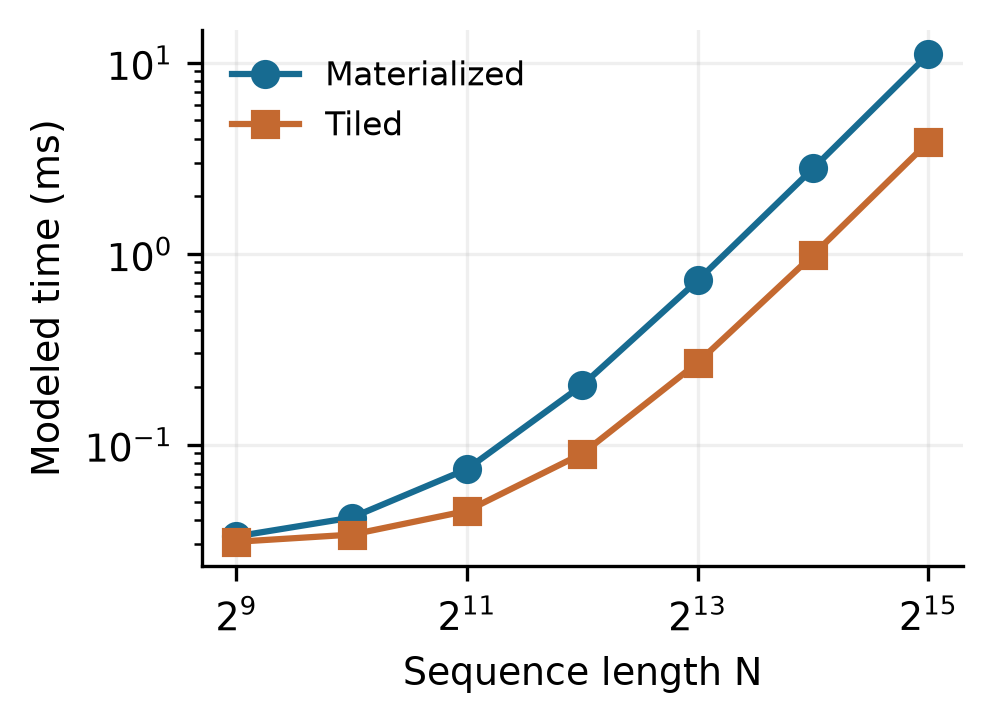
\includegraphics[width=\linewidth]{assets/runtime.png}
 \caption{Synthetic forward-time model at $d=64$. The log axes expose both the launch-dominated region and the larger-workload trend. No hardware measurements are plotted.}
 \label{fig:time}
\end{figure}

An important diagnostic is to inspect the selected component, not only the total. In the materialized schedule, the byte term can dominate while the tiled schedule is limited by arithmetic. In that regime, adding bandwidth to the tiled case provides little benefit within the model. A report that simply attributes every improvement to ``faster memory'' would miss the change in the active constraint.

Table~\ref{tab:results} gives a subset of generated values. Times are rounded for readability, whereas ratios are computed from unrounded model outputs. The table is generated programmatically and is deliberately small: its role is to provide numerical anchors for the curves, not to duplicate every record in the CSV. The full dataset remains available for inspection.

\begin{table}[t]
\caption{Deterministic illustrative outputs for $d=64$. Times include the assumed 30~$\mu$s overhead; these are not measurements.}
\label{tab:results}
\centering
\begin{tabular}{rrrr}
\toprule
$N$ & Materialized (ms) & Tiled (ms) & Ratio \\
\midrule
512 & 0.033 & 0.031 & 1.07 \\
1024 & 0.041 & 0.034 & 1.23 \\
2048 & 0.074 & 0.045 & 1.66 \\
4096 & 0.205 & 0.090 & 2.28 \\
8192 & 0.724 & 0.269 & 2.69 \\
16384 & 2.794 & 0.984 & 2.84 \\
32768 & 11.064 & 3.848 & 2.88 \\
\bottomrule
\end{tabular}
\end{table}


\subsection{Temporary workspace}
Figure~\ref{fig:workspace} uses the separately defined workspace expressions. The materialized curve grows quadratically in $N$, while the tiled expression combines a linear component with a fixed tile term. At smaller shapes, that fixed term matters; at larger shapes, the difference in growth rates becomes the dominant feature. This is a statement about the allocation model, not a measured maximum from a memory profiler.

\begin{figure}[t]
 \centering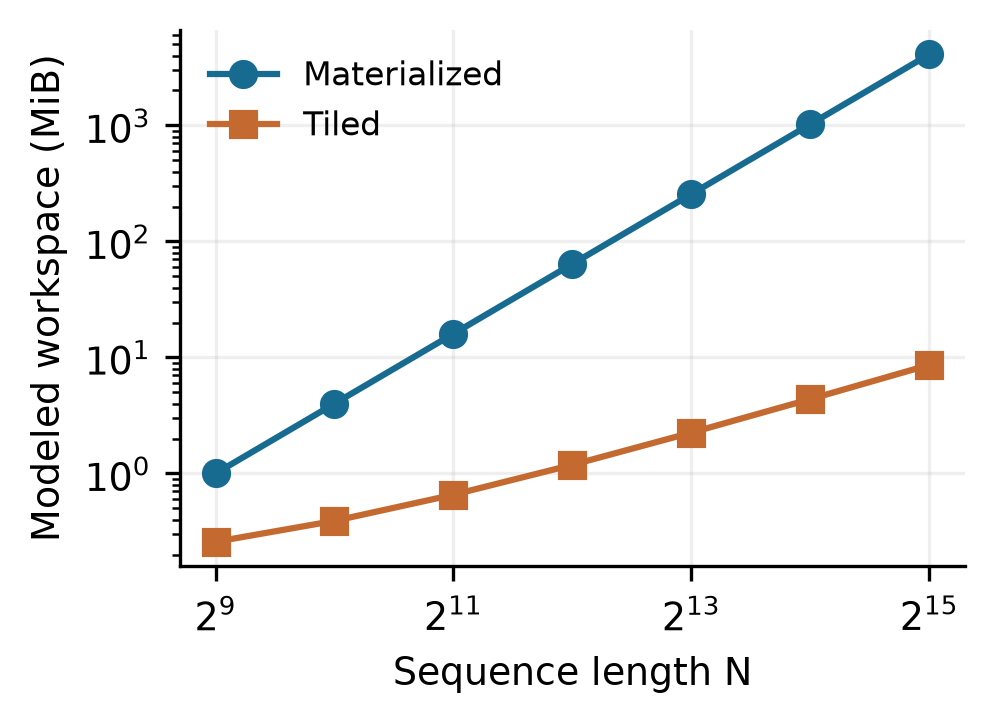
\includegraphics[width=\linewidth]{assets/workspace.png}
 \caption{Synthetic temporary workspace. Inputs, model weights, allocator overhead, and backward state are excluded from both curves. Binary MiB units are used.}
 \label{fig:workspace}
\end{figure}

It would be inappropriate to turn this plot directly into an out-of-memory threshold for a named device. Such a threshold requires a complete accounting of persistent tensors, batch size, framework allocations, and reserve capacity. It also requires the actual allocation policy. Fragmentation or an implementation-specific temporary can change feasibility even when the leading expression remains favorable. The plot instead identifies why a measured study should record peak allocation separately from transferred bytes.

\subsection{The head-dimension dimension}
Figure~\ref{fig:heatmap} expands the comparison across head dimensions. Increasing $d$ raises the shared arithmetic count and the linear traffic terms, while the quadratic traffic difference remains fixed by our coefficients. Consequently, the relative contribution of the traffic reduction changes. A single baseline head dimension cannot represent the whole parameter space even in this simplified setting.

\begin{figure*}[t]
 \centering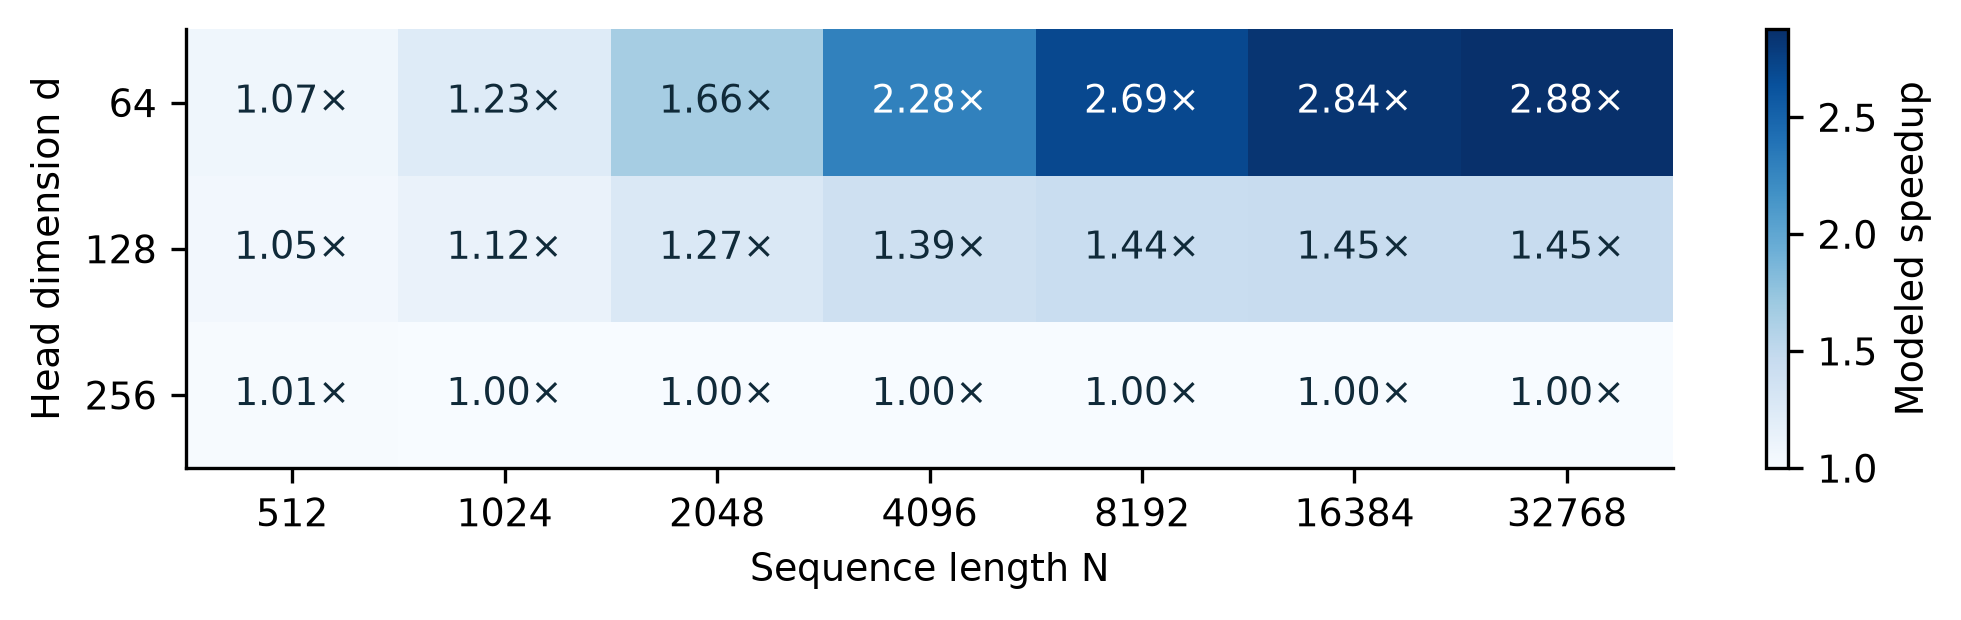
\includegraphics[width=.86\textwidth]{assets/speedup-grid.png}
 \caption{Synthetic speedup across sequence lengths and head dimensions. Each cell is a deterministic ratio from the same model; the colors are not evidence of measurement uncertainty or statistical significance.}
 \label{fig:heatmap}
\end{figure*}

This observation suggests a reporting rule for real studies: shapes should be treated as part of the workload definition, not as incidental benchmark settings. Reporting only the best-performing shape can make an optimization appear more general than the evidence supports. A useful shape sweep includes cases where the improvement is small, as these cases often reveal the limiting mechanism most clearly.

\subsection{Reading a speedup responsibly}
A ratio can obscure the absolute scale of a benefit. A large percentage change on a tiny operation may have little practical effect, while a moderate ratio on a dominant operation can matter greatly. We therefore pair the ratio grid with an absolute-time plot and a workspace plot. Their agreement is not guaranteed; when they tell different stories, the difference is informative.

The model also illustrates why a numerical comparison should not be labeled a benchmark merely because it has axes, legends, and units. The artifact contains a reproducible calculation, but reproducibility alone does not establish empirical validity. All performance language in this section is conditional: it describes what the chosen model predicts, and it identifies what a subsequent experiment would need to test.

\section{Sensitivity and Counterfactual Scenarios}
\label{sec:sensitivity}
A model becomes easier to interpret when its conclusions are tested against changes in its assumptions. We use sensitivity analysis to ask which resource would matter next if one cost were reduced. These are counterfactual scenarios. They do not represent overclocking experiments, measurements on multiple devices, or estimates of future hardware capabilities.

\subsection{Bandwidth sweep}
Figure~\ref{fig:bandwidth} fixes $N=8192$ and $d=64$ while varying the hypothetical bandwidth. The materialized schedule initially benefits from increasing this parameter because transfer is its active component. Once arithmetic dominates, the curve flattens. The tiled schedule can reach that region earlier because its modeled byte count is smaller. The resulting speedup is therefore not constant across hypothetical devices.

\begin{figure}[t]
 \centering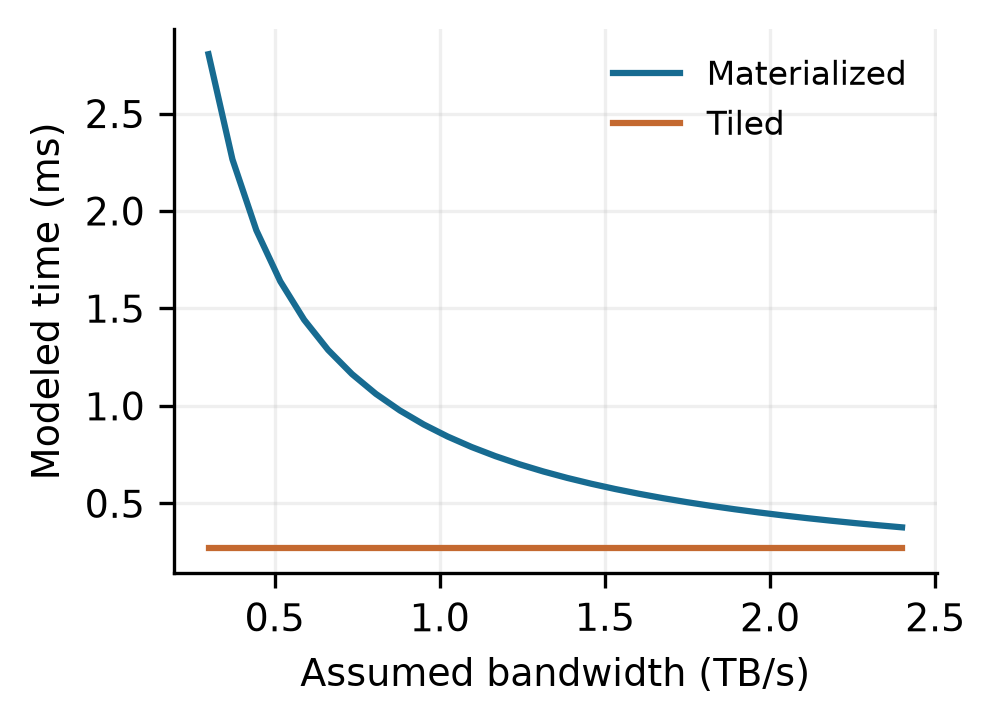
\includegraphics[width=\linewidth]{assets/bandwidth.png}
 \caption{Synthetic bandwidth counterfactual at $N=8192,d=64$. All other assumptions are held fixed. The flat region is a model constraint, not a measured saturation point.}
 \label{fig:bandwidth}
\end{figure}

The crossover has an operational interpretation. If a profiler shows that an implementation is already limited by arithmetic or dependency chains, optimizing a transfer that is fully hidden may not improve elapsed time. Conversely, a reduction in traffic can still improve energy or shared-resource interference, neither of which is represented here. A flat time curve is therefore not evidence that the removed bytes are useless in every system objective; it says that this objective and this model do not value them at that point.

\subsection{Arithmetic efficiency}
Figure~\ref{fig:efficiency} varies the arithmetic fraction while keeping nominal peak throughput fixed. The tiled schedule is more sensitive over the region where arithmetic limits it. This supports a sequential way of thinking about optimization: reducing one bottleneck can expose another. It does not justify assuming that the effective fraction can be raised independently in a real kernel, because occupancy, synchronization, and instruction mix may be coupled.

\begin{figure}[t]
 \centering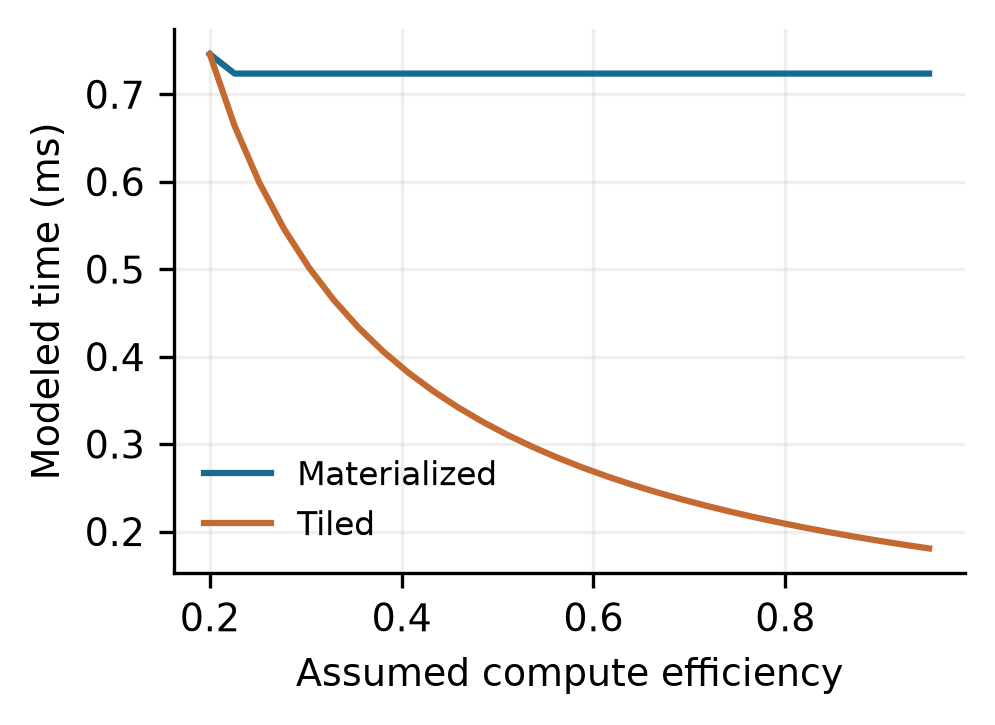
\includegraphics[width=\linewidth]{assets/efficiency.png}
 \caption{Synthetic arithmetic-efficiency sweep. The horizontal axis is an assumed effective fraction of peak, not a reported utilization measurement.}
 \label{fig:efficiency}
\end{figure}

Work-partitioning research makes the distinction between fewer transfers and better execution efficiency particularly relevant~\cite{dao2023flashattention2}. Our model retains only a scalar efficiency parameter, so it cannot distinguish between reasons for low efficiency. Different causes may require opposite implementation changes. A larger tile may improve reuse but increase register demand; more parallel tasks may improve occupancy but require additional synchronization. The scalar is useful for sensitivity, not for diagnosing a kernel.

\subsection{Launch overhead and small workloads}
The launch term bounds the improvement obtainable by changing the resource terms. If both schedules have nearly identical fixed overhead, reducing a small variable cost cannot make the whole operation arbitrarily faster. This behavior is visible in the left side of Figure~\ref{fig:time}. The model does not include fusion across attention and neighboring operators, so it also does not estimate how a different integration boundary would change that overhead.

A future empirical study should report its timing boundary precisely. Host dispatch, device synchronization, graph replay, and batch formation can produce different notions of latency. An author should not compare a device-only timing for one implementation with an end-to-end timing for another. The correct boundary depends on the research question, but it must remain consistent within a comparison.

\subsection{End-to-end limits}
Let $f$ be the fraction of an application's baseline time spent in the modeled attention operation and let $S$ be its local speedup. If everything else is unchanged, the corresponding end-to-end ratio is
\begin{equation}
 S_{\mathrm{end}}=\frac{1}{(1-f)+f/S}.
 \label{eq:end}
\end{equation}
This equation is an accounting identity under the stated decomposition. It does not imply that $f$ is constant when batch size, memory pressure, or scheduling changes. Those interactions can be important, but they require additional evidence rather than an unqualified extrapolation from a kernel result.

For illustration, a local ratio of three and a baseline attention share of one half produce an end-to-end ratio of 1.5. With a share of one fifth, the ratio is only about 1.15. These arithmetic examples are not application measurements. They show why a paper should disclose the attention share before presenting a local improvement as an overall system benefit.

\section{From Illustration to a Measured Study}
\label{sec:discussion}
Turning this artifact into an implementation paper would require new evidence, not merely replacing the word ``synthetic'' in the captions. The first step would be to identify a concrete implementation and a complete workload contract. That contract should specify precision, tensor layout, masking, batch size, head count, sequence-length distribution, and whether the experiment covers forward, backward, prefill, or decoding behavior.

\subsection{Correctness protocol}
A numerical reference should be chosen before tuning performance. Test cases should cover small shapes that can be inspected independently, extreme input magnitudes, non-divisible tile sizes, and masked positions. The report should distinguish absolute error, relative error, and downstream task quality. A test that passes on randomly sampled small tensors may still miss a boundary-condition defect on the longest shape.

The same discipline applies to gradients if backward execution is included. Forward agreement does not establish backward correctness. Tests should document whether they compare analytical gradients, finite differences, or a trusted implementation. Where different accumulation orders are expected, tolerances should be justified and consistently applied rather than adjusted after observing an inconvenient result.

\subsection{Measurement protocol}
Timing should include enough repetitions to characterize variability, with a stated warmup policy and synchronization boundary. Raw samples should be retained, not only their mean. The report should identify the device, driver, runtime, compiler, and library versions so that a future reader can distinguish an algorithmic change from a changed execution environment. Clock or power settings should be described when they are controlled.

For resource measurements, the selected tool and its counter definitions matter. An observed memory-transaction count is not automatically equivalent to the abstract bytes in Equation~\ref{eq:bytes}. Cache effects, compression, transaction granularity, and profiling overhead can alter the relationship. A measured study should explain how a counter is mapped to the claimed quantity and should avoid combining counters collected under incompatible conditions.

\subsection{Fair baselines and integration}
Baselines should solve the same problem with comparable precision and masking semantics. They should receive reasonable configuration effort, and any unsupported shapes should be disclosed. An optimization that changes the workload contract may still be useful, but it belongs in a different comparison. Reporting both absolute values and ratios makes those differences harder to hide.

Integration tests should complement isolated kernels. Allocation policy, graph capture, scheduling, and neighboring operations can change the effective workload seen by the kernel. Serving systems add another layer: the distribution of requests and the cache-management policy can dominate the useful throughput of a deployment. The context of PagedAttention illustrates why serving-memory management deserves an explicit experimental boundary~\cite{kwon2023pagedattention}, rather than being folded into a generic statement about attention speed.

\subsection{Limitations of this artifact}
Our byte coefficients are illustrative, the overlap assumption is optimistic, and the effective rates are not calibrated. We omit batch interactions, backward state, detailed numerical behavior, and device-specific scheduling. The model also cannot predict energy consumption, tail latency, or fairness among concurrent requests. Any of those objectives would require its own variables and measurements.

The document itself has limitations. It is a demonstration of a scholarly workflow, not a peer-reviewed research contribution. Its author label is a project label rather than a real researcher identity. The ACM class supplies familiar typography, but neither that typography nor successful compilation implies ACM endorsement, publication, or compliance with a particular conference's current submission requirements. Keeping these limits explicit is part of the artifact's design.

\subsection{What a negative result would mean}
If a future implementation failed to achieve the qualitative model trend, that would not automatically invalidate IO awareness. It could indicate that a neglected cost dominates, that the traffic coefficient is unrealistic, or that the implementation exposes insufficient parallelism. The useful response would be to measure the missing mechanism and revise the model. A model is a tool for organizing questions, not an authority that an implementation must obey.

\section{Conclusion}
\label{sec:conclusion}
This demonstration separates an attention expression, a storage schedule, a synthetic performance model, and an actual authoring artifact. The separation is the main lesson. Fewer transferred bytes, lower temporary workspace, and shorter elapsed time are different claims that require different evidence. A compact model can make their relationship visible, provided its assumptions remain attached to its results.

The numerical study shows how launch overhead can limit small-workload improvements, how arithmetic can become the active constraint after traffic is reduced, and how shape and resource assumptions change a ratio. These are conditional consequences of the specified model. They are not measured accelerator results and should not be cited as such. The project supplies a reproducible starting point for further analysis, including the source data, figures, BibTeX records, and compiled PDF; the companion generator is included in the project tools directory.

A substantive next step would be to replace the abstract schedules with validated implementations and collect measurements under a documented protocol. Until then, the artifact is useful as a reasoning aid and a demonstration of transparent scientific authoring. Its value comes from making the boundary between illustration and evidence easy to inspect.

\bibliographystyle{ACM-Reference-Format}
\bibliography{references}
\appendix
\section{Reproduction and Audit Guide}
\label{sec:appendix}
This appendix explains how to reproduce the artifact and how to inspect its boundaries. It is a guide to a deterministic calculation, not instructions for recreating a GPU experiment. The source directory contains the manuscript, bibliography, and generated CSV records. A companion development tool retains the figure generator and its explicit input assumptions. The build directory contains the rendered manuscript and its compilation log. Generated outputs can be replaced without changing the source of the calculation.

\subsection{Artifact inventory}
The entry point is \texttt{main.tex}. The files in \texttt{chapters/} separate background, model, experimental design, illustrative evaluation, sensitivity analysis, and discussion. This division is editorial: the compiler follows the explicit input statements in the entry point. A file that is present in the directory but not reachable from those statements does not automatically become part of the paper.

The companion figure generator (kept in the application development tools) uses Python, NumPy, and Matplotlib. Running it from any working directory writes six high-resolution PNG figures and retained vector sources, a numeric CSV, and a small LaTeX table into the demonstration project. The calculations use double-precision floating-point arithmetic. There is no random seed because no random quantity is sampled. Version information belongs in the accompanying reproduction notes so that changes in rendering can be distinguished from changes in the numeric model.

The CSV records identify the sequence length and head dimension, followed by the arithmetic count, traffic estimates, component times, total times, and temporary workspace. These fields allow a reader to reconstruct each chart without extracting values from a plotted line. A derived ratio is obtained by dividing the two total-time fields; it is not an independently estimated parameter. A rounded value in the manuscript should therefore be checked against the unrounded CSV rather than against another rounded value.

\subsection{A worked arithmetic check}
Consider $N=8192$ and $d=64$. The shared arithmetic count is $17{,}179{,}869{,}184$ operations under Equation~\ref{eq:flops}. The materialized traffic expression gives $541{,}065{,}216$ bytes, while the tiled expression gives $37{,}748{,}736$ bytes. With the stated effective rates, the arithmetic component is approximately $0.239$ milliseconds. The two transfer components are approximately $0.694$ and $0.048$ milliseconds. Taking the maximum and then adding the overhead yields approximately $0.724$ and $0.269$ milliseconds. The resulting ratio is approximately $2.69$.

These numbers are arithmetic consequences of the assumptions. In particular, the lower transfer estimate does not cause the tiled total to fall to $0.078$ milliseconds: the shared arithmetic component is larger. This worked example exposes a common interpretive error, namely comparing only the transfer terms after the active constraint has changed. It also explains why the table uses a maximum rather than adding both components together.

For the same shape, the materialized workspace estimate is $268{,}435{,}456$ bytes, or $256$ MiB. The tiled estimate is $2{,}359{,}296$ bytes, or $2.25$ MiB. Neither number includes model weights or the input tensors. A reader should not add one of these numbers to an unrelated profiler result without checking whether the two quantities count overlapping allocations.

\subsection{Unit conventions}
The assumed transfer rate uses decimal terabytes per second: one TB/s is $10^{12}$ bytes per second. Workspace plots use binary mebibytes: one MiB is $2^{20}$ bytes. These conventions are deliberately stated separately. Replacing a decimal rate with a binary rate while keeping the same numerical coefficient would alter the computed time. The difference is modest relative to the model's conceptual limitations, but a reproducible calculation should still avoid silent unit changes.

The operation count uses a multiply-add convention in which the two dominant matrix products together contribute $4N^2d$ operations. Softmax arithmetic and address calculations are not separately counted. This omission is part of the model definition, not evidence that their cost is zero. A more detailed simulator could add these components, but the resulting parameters would need new justification.

\subsection{Invariants worth checking}
All byte counts, workspaces, and component times must be positive for the positive shapes in the sweep. The total time must be no smaller than the fixed overhead and no smaller than either selected component plus that overhead. The two schedules share exactly the same arithmetic count for a given shape. Consequently, a reduction in byte traffic cannot push either total below its common arithmetic floor.

The materialized traffic is greater than the tiled traffic for every positive $N$ because their difference is $7.5N^2$ bytes. With identical efficiencies and launch terms, the model therefore cannot predict a tiled slowdown. This is an imposed property of the comparison and an especially important limitation. A real implementation may experience lower occupancy, more instructions, different synchronization, or a fallback path. The absence of slowdowns in this dataset does not demonstrate their absence in practice.

A useful audit modifies one assumption at a time. Increasing only bandwidth cannot increase either predicted total. Increasing only compute efficiency cannot increase either total. Increasing the fixed overhead by a common positive amount moves the ratio closer to one. These checks exercise the meaning of the equations and can catch unit errors or a swapped variable without relying on a reference picture.

\subsection{Extending the model without obscuring it}
A next version could assign different compute efficiencies to the two schedules. That change would allow the tiled schedule's arithmetic cost to trade off against its lower traffic. The revised experiment should present both the original common-efficiency comparison and the new comparison so that the source of any reversal remains visible. An unexplained efficiency adjustment selected to match a preferred ratio would weaken the artifact rather than improve it.

A second extension could replace the maximum with an overlap parameter. Perfect overlap and complete serialization provide different limiting cases. Such a parameter should be bounded and interpreted physically; it should not become an arbitrary curve-fitting knob. The report should include the limiting cases and identify which observable would constrain the parameter in a real measurement.

A third extension could model causal attention explicitly. The current square score domain is the same for both schedules and does not claim a triangular execution count. Halving one coefficient without changing the rest would not produce a complete causal model. Arithmetic, transfer, masking, and scheduling would all need compatible definitions. The same caution applies to variable sequence lengths and padding removal.

\subsection{A prospective measurement worksheet}
Before replacing synthetic values with measured values, define the workload contract. Record whether the operation is forward-only or includes gradients, whether attention is causal, the input dtype, accumulation behavior, batch size, head count, sequence lengths, and tensor layout. Record the library and compiler versions together with the device and runtime. These fields identify the experiment; none is supplied by the present CSV.

Next, establish numerical correctness with a suitable reference. Record both absolute and relative error and explain how zero or near-zero reference values are handled. Test representative shapes and edge cases separately. A timing result from an incorrect path should not be averaged into an otherwise correct benchmark. A fallback implementation should be labeled because it may use a different schedule from the one being studied.

Then specify the timing boundary. Decide whether allocations, input transfer, graph capture, and synchronization are included. Use a synchronization method appropriate to asynchronous execution, and document warmup separately from collected trials. Preserve the individual measurements needed to examine variability. A single best time is inadequate for characterizing stability, while a mean without a distribution can hide occasional expensive paths.

Finally, record memory quantities with their definitions. Allocated bytes, reserved bytes, maximum temporary workspace, and traffic inferred from performance counters are different observations. A counter may include transactions that are not represented by a simple tensor-size formula. A discrepancy between a counter and the model should start an investigation of definitions and mechanisms before being described as a failed optimization.

\subsection{Reviewing claims and citations}
Each citation should support a specific statement. The bibliography in this demonstration contains identifiable public research records, while the synthetic model is introduced as the artifact's own construction. The numerical plots should not be attributed to those records. Conversely, the existence of this small model is not a basis for claiming a new attention algorithm or a new empirical result.

An editorial review can make three separate checks. References should resolve to the intended records. The prose should separate prior work from the illustrative calculation. Every numerical claim should be traceable to an equation or generated data. Correct bibliography formatting alone addresses only the first layer. A professionally formatted PDF can still make unsupported claims, so presentation quality and evidential quality should be evaluated separately.

\subsection{Build and version boundaries}
A successful build verifies that the TeX inputs, bibliography, and figure paths resolve together. It does not verify the scientific interpretation. The local build uses the installed ACM class in its non-publication mode, with no invented conference identity or copyright statement. The author line identifies the demonstration rather than a fictional research team. This makes the artifact useful for exercising a writing interface without impersonating a submitted paper.

Source files and figure inputs are suitable for version control. Temporary TeX files and generated manuscript output belong in the ignored build directory. Input PDF figures remain eligible for tracking because the manuscript depends on them. Initializing a repository creates a version-control container; it does not create a commit, establish authorship, or publish the paper. A user can decide when a coherent revision is ready to commit and whether a release PDF should later be attached to a tagged version.

\end{document}
